% --------------------------------------------------------------
% This is all preamble stuff that you don't have to worry about.
% Head down to where it says "Start here"
% --------------------------------------------------------------

\documentclass[12pt]{article}

\usepackage[margin=1in]{geometry}
\usepackage{times}
\usepackage{amsmath,amsthm,amssymb}
\usepackage{caption}
\usepackage{graphicx,subfigure}
\usepackage{listings}
\usepackage{url}

\newcommand{\N}{\mathbb{N}}
\newcommand{\Gauss}{\mathcal{N}}
\newcommand{\Z}{\mathbb{Z}}
\newcommand{\E}{\mathbb{E}}
\newcommand{\R}{\mathbb{R}}
\newcommand{\p}{{\bf p}}
\newcommand{\1}{\mathbf{1}}

% \linespread{0}

\newenvironment{theorem}[2][Theorem]{\begin{trivlist}
\item[\hskip \labelsep {\bfseries #1}\hskip \labelsep {\bfseries #2.}]}{\end{trivlist}}
\newenvironment{lemma}[2][Lemma]{\begin{trivlist}
\item[\hskip \labelsep {\bfseries #1}\hskip \labelsep {\bfseries #2.}]}{\end{trivlist}}
\newenvironment{claim}[2][Claim]{\begin{trivlist}
\item[\hskip \labelsep {\bfseries #1}\hskip \labelsep {\bfseries #2.}]}{\end{trivlist}}
\newenvironment{exercise}[2][Exercise]{\begin{trivlist}
\item[\hskip \labelsep {\bfseries #1}\hskip \labelsep {\bfseries #2.}]}{\end{trivlist}}
\newenvironment{problem}[2][Problem]{\begin{trivlist}
\item[\hskip \labelsep {\bfseries #1}\hskip \labelsep {\bfseries #2.}]}{\end{trivlist}}
\newenvironment{question}[2][Question]{\begin{trivlist}
\item[\hskip \labelsep {\bfseries #1}\hskip \labelsep {\bfseries #2.}]}{\end{trivlist}}
\newenvironment{corollary}[2][Corollary]{\begin{trivlist}
\item[\hskip \labelsep {\bfseries #1}\hskip \labelsep {\bfseries #2.}]}{\end{trivlist}}

\begin{document}
{\raggedright

% --------------------------------------------------------------
%                         Start here
% --------------------------------------------------------------

\title{ECE 544NA HW3}%replace X with the appropriate number
\author{Jiaqi Mu~jiaqimu2 \\
% collaborating with Hongyu Gong~hgong6 \\
[8pt]%replace with your name
Department of Electrical and Computer Engineering} %if necessary, replace with your course title

\maketitle

\section{Pencil-and-Paper\label{sec:1}}

In this portion of the assignment, you will derive the update equations for a binary-binary RBM. Let $(V, H)$ denote the visible and hidden random variable which takes values ($v\in \{0,1\}^{m}$, $h\in \{0,1\}^n$). Then the joint probabolity distribution is described by the distribution $p(v, h;\theta) = \frac{1}{Z} e^{-E(v, h;\theta)}$, where $E$ is the following energy function,
\begin{align*}
  E(v, h; \theta) &= -\sum_{i=1}^n \sum_{j=1}^m w_{ij} h_iv_j - \sum_{j=1}^m b_j v_j - \sum_{i=1}^n c_i h_i \\
  &= -(v^{\rm T}W h + v^{\rm T}b + h^{\rm T}c),
\end{align*}
where $Z = \sum_{v}\sum_{h} e^{-E(v, h; \theta)}$, and $\theta = (W, b,c)$.
\begin{itemize}
  \item Find $p(v|h,\theta)$ and $\E(v|h, \theta)$. Show that $p(v_j|h)$ has the form $sigmoid\left(\sum_{i=1}^n w_{ij} h_i + b_j\right)$.
  \begin{proof}
  Given the joint distribution, one knows the conditional distribution as,
  \begin{align*}
    p(v|h, \theta) &= \frac{p(v,h;\theta)}{p(h; \theta)} \\
    &= \dfrac{e^{-E(v, h;\theta)}}{\sum_{u} e^{-E(u, h; \theta)}} \\
    &= \dfrac{e^{v^TWh + v^Tb + h^Tc}}{\sum_{u} e^{{u}^TWh + {u}^Tb + h^Tc}} \\
    &= \dfrac{1}{\sum_u e^{(u-v)^T W h + (u-v)^T b}} \\
    &= \dfrac{1}{\sum_u e^{(u-v)^T (Wh + b)}} \\
    &= \dfrac{1}{\prod_{j=1}^m \left(1 + e^{-(2v_j - 1)(W_j^{\rm T}h + b_j)}\right)},
  \end{align*}
  where $W_j$ is the $j$-th row of $W$. Specially, we can see $p(v|h, \theta)$ can be factorized as,
  \begin{align*}
    p(v|h, \theta) &= \prod_{j=1}^m \frac{1}{1 + e^{-(2v_j - 1)(W_j^{\rm T}h + b_j}}.
  \end{align*}
  Thus, given $h$, $v_1$,...,$v_m$ are conditionally independent, thus,
  \begin{align*}
    p(v_j|h, \theta) = \frac{1}{1 + e^{-(2v_j - 1)(W_j^{\rm T}h + b_j}} = \left\{\begin{array}{ll} \frac{1}{1 + e^{-(\sum_{i=1}^n w_{ij}h_i + b_j)}} & v_j = 1 \\ \frac{1}{1 + e^{\sum_{i=1}^n w_{ij}h_i + b_j}} & v_j = 0\end{array}\right..
  \end{align*}
  The conditional expectation is thus given as,
  \begin{align*}
    \E(v | h; \theta) = \left(E(v_1|h; \theta) ,..., \E(v_n | h; \theta ) \right), 
  \end{align*}
  where $\E(v_j|h; \theta)$ is given as,
  \begin{align*}
    \E(v_j|h; \theta) = p(v_j=1|h; \theta) = sigmoid\left(\sum_{i=1}^n w_{ij}h_i + b_j\right).
  \end{align*}
  \end{proof}
  \item Find $p(h|v; \theta)$ and $E(h|v; \theta)$. Show that $p(h_i|v)$ has the form $sigmoid(\sum_{j=1}^m w_{ij} v_j + c_i)$.
  \begin{proof}
    In $E(v, h; \theta)$, $v$ and $h$ are symmetric, thus following the steps in part 1 we know,
    \begin{align*}
      p(h | v; \theta) = \prod_{i=1}^n \frac{1}{1 + e^{-2(h_i - 1)(v^{\rm T} W_i + c_i)}},
    \end{align*}
    where $W_i$ is the $i$-th column of $W$. The conditional distribution and the conditional expectation are,
    \begin{align*} 
      \E(h_i; v; \theta) &= sigmoid\left(\sum_{j=1}^m w_{ij} v_j + c_i\right) \\
      P(h_i | v; \theta) &= \left\{\begin{array}{ll}\frac{1}{1 + e^{-(\sum_{j=1}^m w_{ij} v_j + c_i) }} & h_i = 1 \\ \frac{1}{1 + e^{\sum_{j=1}^m w_{ij} v_j + c_i}} & h_i = 0 \end{array}\right.
    \end{align*}
  \end{proof}
  \item Now you are given a dataset of $D = \{v_1,...,v_N\}$. The log-likelihood of the dataset can be computed as,
  \begin{align*}
    \mathcal{L}(D | \theta) = \sum_{t=1}^N \log (p(v_t | \theta)).
  \end{align*}
  Compute $\frac{\partial \mathcal{L}(D|\theta)}{\partial \theta}$, and express it in terms of $p(h|v)$, $p(h, v)$ and $\frac{\partial E(v,h)}{\partial \theta}$.
  \begin{proof}
    First we compute $p(v; \theta)$. This can be computed via $p(v, h; \theta)$, i.e.,
    \begin{align*}
      p(v;\theta) = \sum_{h} p(v, h) = \frac{1}{Z} e^{-F(v)},
    \end{align*}
    where $F(v)$ is defined to be $F(v) = -\log \sum_h e^{-E(v, h;\theta)}$, and $Z$ is the partition function defined as $Z = \sum_v e^{-F(v)}$, and can be simplified as,
    \begin{align*}
      F(v) &= - \log \sum_h e^{(v^{\rm T} W h + v^{\rm T} b + h^{\rm T} c)} \\
      &= - \log e^{v^{\rm T} b} \sum_{h} e^{(W^{\rm T} v + c)^{\rm T} h} \\
      &= - \log e^{v^{\rm T} b} \prod_{i=1}^n (1 + e^{v^{\rm T} W_i + c_i}) \\
      &= - v^{\rm T} b - \sum_{i=1}^n \log (1 + e^{v^{\rm T} W_i + c_i}).
    \end{align*}
    Based on the chain rule, the answer is given as follow,
    \begin{align*}
      \frac{\partial \mathcal{L}(D|\theta)}{\partial \theta} = \sum_{t=1}^N \frac{\partial}{\partial \theta} \log p(v_t | \theta),
    \end{align*} 
    where,
    \begin{align*}
      \frac{\partial \log p(v | \theta)}{\partial \theta} &= \frac{\partial}{\partial \theta} \left(-F(v) - \log Z\right) \\
      &= -\frac{\partial F(v)}{\partial \theta} - \frac{1}{Z}\sum_u \frac{\partial e^{-F(u)}}{\partial \theta} \\
      &= -\frac{\partial F(v)}{\partial \theta} + \sum_u \frac{e^{-F(u)}}{Z} \frac{\partial F(u)}{\partial \theta} \\
      &= -\frac{\partial F(v)}{\partial \theta} + \sum_u p(u) \frac{\partial F(u)}{\partial \theta}.
    \end{align*}
    As required, $\frac{\partial \log p(v | \theta)}{\partial \theta}$ can also be written as,
    \begin{align*}
      \frac{\partial \log p(D | \theta)}{\partial \theta} = -\sum_{t=1}^N \sum_h p(h|v_t; \theta) \frac{\partial E(v_t,h; \theta)}{\partial \theta} + N \sum_v \sum_h p(v,h ; \theta) \frac{\partial E(v,h)}{\partial \theta}.
    \end{align*}
  \end{proof}
    \item Use the result in (2) compute $\frac{\partial \mathcal{L}(D|\theta)}{\partial W_{ij}}$, $\frac{\partial \mathcal{L}(D|\theta)}{\partial b_j}$ and $\frac{\partial \mathcal{L}(D|\theta)}{c_i}$.
    \begin{proof}
      Given $F(v)$, we know,
      \begin{align*}
        \frac{\partial F(v; \theta)}{\partial W_{ij}} &= -\sum_{i=1}^n \frac{1}{1 + e^{v^T W_i + c_i }} \frac{\partial e^{v^T W_i + c_i }}{\partial W_{ij}} = - \frac{1}{1 + e^{ - (v^T W_i + c_i)}}v_j \\
        &= - v_j sigmoid(v^T W_i + c_i). \\
        \frac{\partial F(v; \theta)}{\partial b_j} &= -v_j \\
        \frac{\partial F(v; \theta)}{\partial c_i} &= --\sum_{i=1}^n \frac{1}{1 + e^{v^T W_i + c_i }} \frac{\partial e^{v^T W_i + c_i }}{\partial c_i} = - \frac{1}{1 + e^{ - (v^T W_i + c_i)}}v_j \\
        &= -sigmoid(v^{\rm T} W_i + c_i).
      \end{align*}
      Thus assembling those together will give,
      \begin{align*}
        \frac{\partial \mathcal{L}(D|\theta)}{\partial W_{ij}} &= \sum_{t=1}^N \left(v_j^{(t)} sigmoid((v^{(t)})^{\rm T}W_i + c_i)  - \E_{v} \left( v_j sigmoid(v^{\rm T} W_i + c_j)\right)\right)  \\
        &= \sum_{t=1}^N \left( v_j^{(t)} sigmoid((v^{(t)})^{\rm T}W_i + c_i)\right)  - N\E_{v, h}(v_j h_i) \\
        \frac{\partial \mathcal{L}(D|\theta)}{\partial b_j} &= \sum_{t=1}^N \left(v_j^{(t)} - \E_v (v_j)\right) \\
        &= \sum_{t=1}^N v_j^{(t)}  - N \E_{v, h}(v_j)) \\
        \frac{\partial \mathcal{L}(D|\theta)}{c_i} &= \sum_{t=1}^N \left( sigmoid((v^{(t)})^{\rm T} W_i + c_i) - \E_v(sigmoid(v^{\rm T} W_i + c_i)) \right) \\
        &= \sum_{t=1}^N \left( sigmoid((v^{(t)})^{\rm T} W_i + c_i)  \right)- N\E_{v, h}(h_i)
      \end{align*}
    \end{proof}
    \item The update equations in (3) contain computationally intractable terms, which ones are intractable? And how do we approximate those terms?
    \begin{proof}
      The computationally intractable terms come from conditional expectations, where the expectation is over all $h$ and $v$. We estimate those by contrastive divergence. Let $\hat{h}$ be the hidden state in the current iteration: 
      \begin{itemize}
        \item $W_{ij}$: $\E_{h,v}(v_jh_i)$ is estimated by,
        \begin{align*}
          \E_{h,v}(v_jh_i) &= \E_h(h_i\E_{v|h}(v|h)) = \E_{h}(h_ip(v_j=1|h; \theta)) \approx \hat{h}_i p(v_j=1|\hat{h}; \theta) \\
          &= \hat{h}_i sigmoid(W_j^{\rm T} \hat{h} + b_j).
        \end{align*}
        \item $b_j$: $\E_{v,h}(v_j)$ is estimated by,
        \begin{align*}
          \E_{h,v}(v_j) &= \E_h(\E_{v|h}(v|h)) = \E_{h}(p(v_j=1|h; \theta)) \approx p(v_j=1|\hat{h}; \theta) \\
          &= sigmoid(W_j^{\rm T} \hat{h} + b_j).
        \end{align*}
        \item $c_i$: $\E_{v,h}(h_j)$ is estimated by $\hat{h}_j$.
      \end{itemize}
      Thus the gradients are,
      \begin{align*}
        \left\{ \begin{array}{ll}
          \frac{\partial \mathcal{L}(D|\theta)}{\partial W_{ij}} = \sum_{t=1}^N \left( v_j^{(t)} sigmoid((v^{(t)})^{\rm T}W_i + c_i)  -  \hat{h}_i^{(t)} sigmoid(W_j^{\rm T} \hat{h}^{(t)} + b_j) \right)\\
          \frac{\partial \mathcal{L}(D|\theta)}{\partial b_j} = \sum_{t=1}^N \left( v_j^{(t)} -  sigmoid(W_j^{\rm T} \hat{h}^{(t)} + b_j) \right)\\
          \frac{\partial \mathcal{L}(D|\theta)}{\partial c_i} =\sum_{t=1}^N \left( sigmoid((v^{(t)})^{\rm T} W_i + c_i)   - \hat{h}_j^{(t)}\right).
        \end{array}\right.
      \end{align*}
    \end{proof}
\end{itemize}

\section{Code-From-Scratch}
In this portion of the assignment, you will write a binary RBM and train on the MNIST dataset. The MNIST dataset contains $28\times 28 \times 1$ image, reshape this into $784\times 1$ vector, this is $v$. Choose $h$ to be of dimension 200. Use the update equations you derived in the pencil-and-paper part to train a RBM. 

\subsection{Methods}
\begin{itemize}
  \item Describe the functions you wrote, and the overall structure of your code.
  \begin{proof}
    In this part I wrote two files, {\tt part2.py} to implement required plots and {\tt rbm\_part2.py} to implement a restricted Boltzmann machine class. In this class, three modules are implemented:
    \begin{itemize}
      \item {\tt \_\_init\_\_}: to initialize parameters, e.g., step size, iteration numbers, batch size, etc.
      \item {\tt fit}: to fit data and train paramters
      \item {\tt getWeights}: to return the learned filters.
    \end{itemize}
  \end{proof}
\end{itemize}

\subsection{Results}
\begin{itemize}
  \item Provide a figure, showing any 64 of the 200 learned filter.
  \begin{proof}
    As in Figure~\ref{fig:part2}.
    \begin{figure}
      \centering
      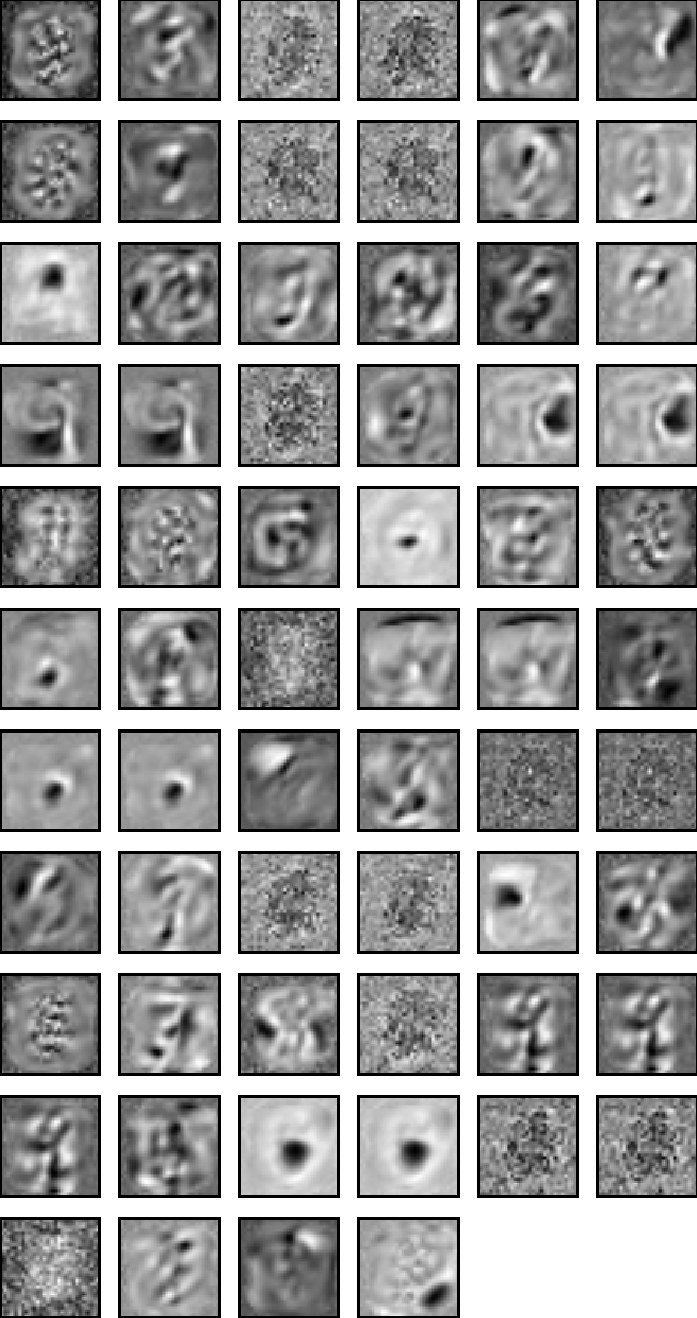
\includegraphics[width=0.7\textwidth]{../figures/part2-filters.pdf}
      \caption{64 filters obtained from RBM.\label{fig:part2}}
    \end{figure}
  \end{proof}
\end{itemize}


\section{TensorFlow}
In this portion of the assignment, you will use RBM, stack of RBM, and PCA to perform dimension reduction on the raw pixels of the MNIST dataset. From the dimension reduced features, you will perform 10-way classification using multi-class logistic regression. 

Report training and testing accuracy for the following:

\begin{itemize}
  \item Train a 10-way multi-class logistic regression on the raw-pixel data.
  \item Train a RBM with 200 hidden units. Perform 10-way multi-class logistic regression on this reduced dimension of 200.
  \item Use PCA to reduce the input dimension to 200. Perform 10-way multi-class logistic regression on this reduced dimension.
  \item Train a stacking of RBMs, with hidden units [500, 200] (i.e. train a RBM with 500 hidden units, then use the output of the first RBM to train a second RBM with 500 hidden units. Perform 10-way multi-class logistic regression on this reduced dimension.
\end{itemize}
For the classification part, you are allowed you use higher-level API such as TFLearn\footnote{\url{http://tflearn.org/}}. This will greatly reduced the amount of code you need to write. 

\subsection{Methods}
\begin{itemize}
  \item Describe the RBM and multi-class logistic regression architecture, discuss how you used TensorFlow functions to create such architecture. Make sure your description matches your code;
  \begin{proof}
    We construct two classes {\tt RMB} and {\tt Logistic} in two files {\tt rmb.py} and {\tt logistic\_regression.py} respectively. The {\tt Logistic} class is the same as the one implemented in homework 1.

    The {\tt RMB} class contains following modules:
    \begin{itemize}
      \item {\tt \_\_init\_\_}: to initialize hyperparamters
      \item {\tt nextBatch}: to generate next batch index
      \item {\tt fit}: to fit and train the input data. We realize this function via following modules:
      \begin{itemize}
        \item {\tt build\_model}: to build the overall graph model for binary binary restricted boltzmann machine
        \item {\tt initialize\_tf}: to initialize all tensorflow variables and tensors.
        \item {\tt train\_model}: to update variables for each batch, where we use {\tt assign\_add} to assign a specific value to update parameters manually.
      \end{itemize}
      \item {\tt transform}: to transform data into hidden layer
    \end{itemize}
  \end{proof}
  \item Report the total number of weights in the stacked RBM.
  \begin{proof}
    The number of parameters in the first layer is
    \begin{align*}
      500 * 784 + 500 + 784 = 393284.
    \end{align*}
    The number of parameters in the second layer is,
    \begin{align*}
      500 * 200 + 500 + 200 = 100700.
    \end{align*}
    The total number of weights in the stacked RBM is,
    \begin{align*}
      393284 + 100700 = 493984.
    \end{align*}
  \end{proof}
\end{itemize}

\subsection{Results}
\begin{itemize}
  \item Provide a table, showing the training and testing accuracy for each of the methods mentioned above.
  \begin{proof}
    The accuracy is provided in Table~\ref{tb:part3}.
    \begin{table}[h]
      \centering
      \begin{tabular} {r|c|c|c|c}
        \hline 
        & raw & pca & RBM-200 & RBM-500-200 \\
        \hline
        train & 92.30 & 92.44 & 84.80 & 90.27 \\
        test & 92.35 & 92.12 & 85.47 & 89.47 \\
        \hline
      \end{tabular}
      \caption{Accuracy for four different models.\label{tb:part3} }
    \end{table}
  \end{proof}
  \item Plot training and testing classification confusion matrix for each of the methods mentioned above.
  \begin{proof}
    The figures for training and testing are plotted in Figure~\ref{fig:part3}.
    \begin{figure}[h]
      \centering
      \subfigure[train-raw]
      {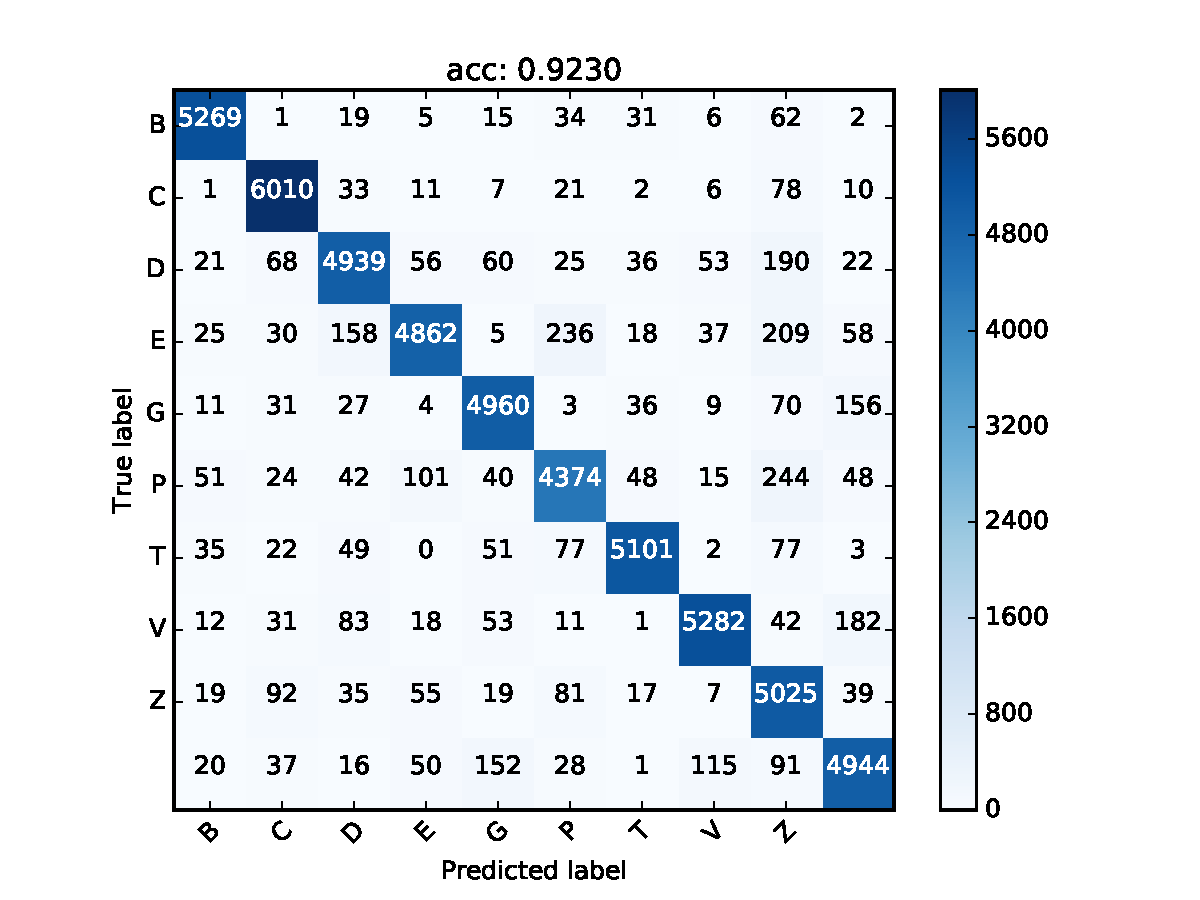
\includegraphics[width = 0.35\textwidth]{../figures/train-raw.pdf}}
      \subfigure[test-raw]
      {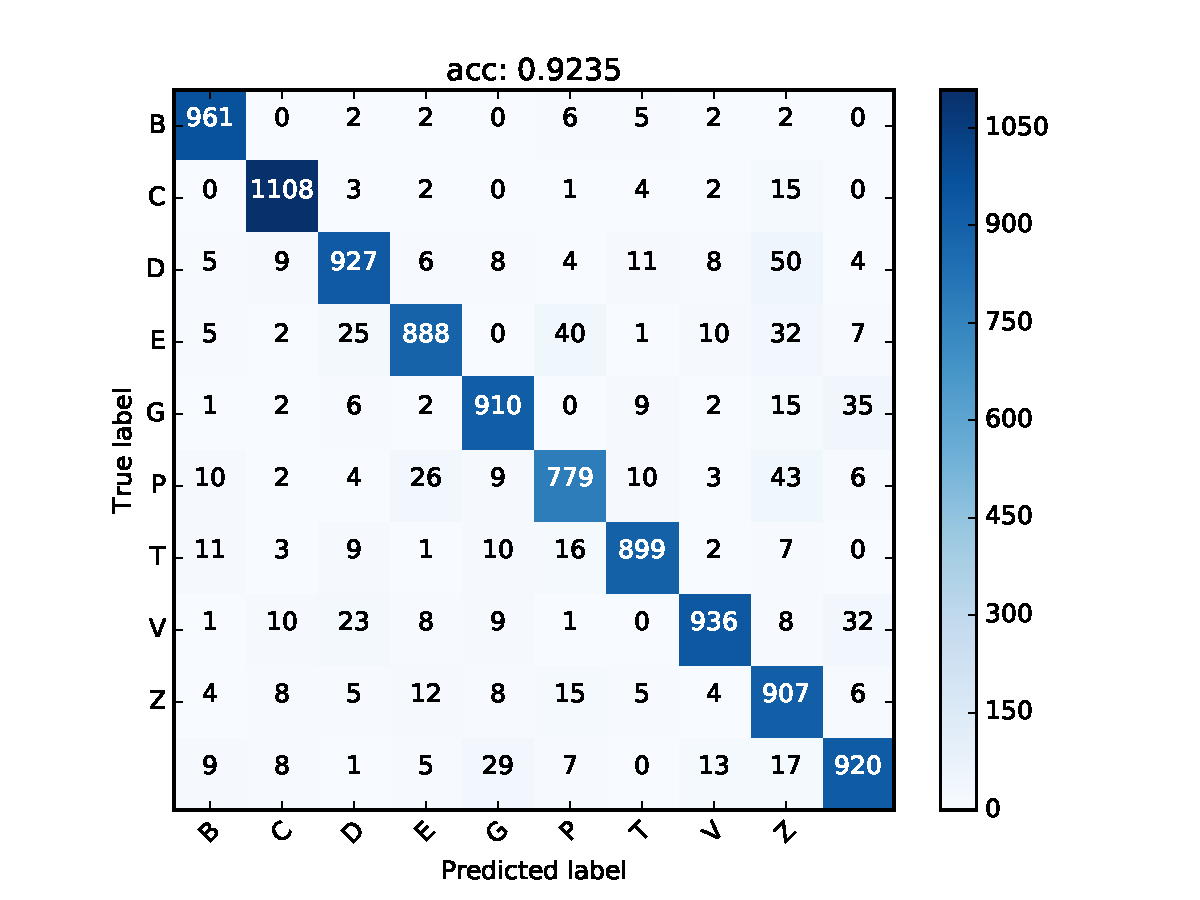
\includegraphics[width = 0.35\textwidth]{../figures/test-raw.pdf}}
      \subfigure[train-pca]
      {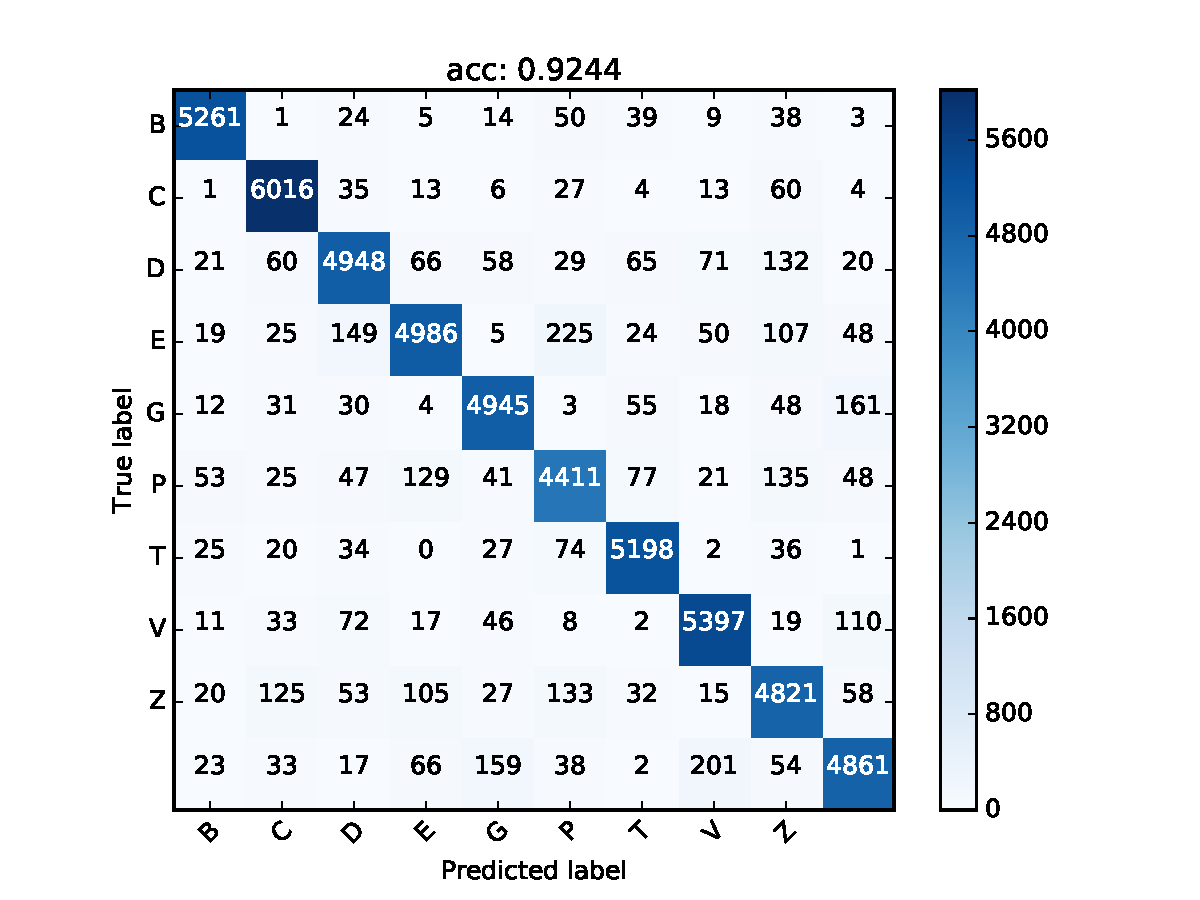
\includegraphics[width = 0.35\textwidth]{../figures/train-pca.pdf}}
      \subfigure[test-pca]
      {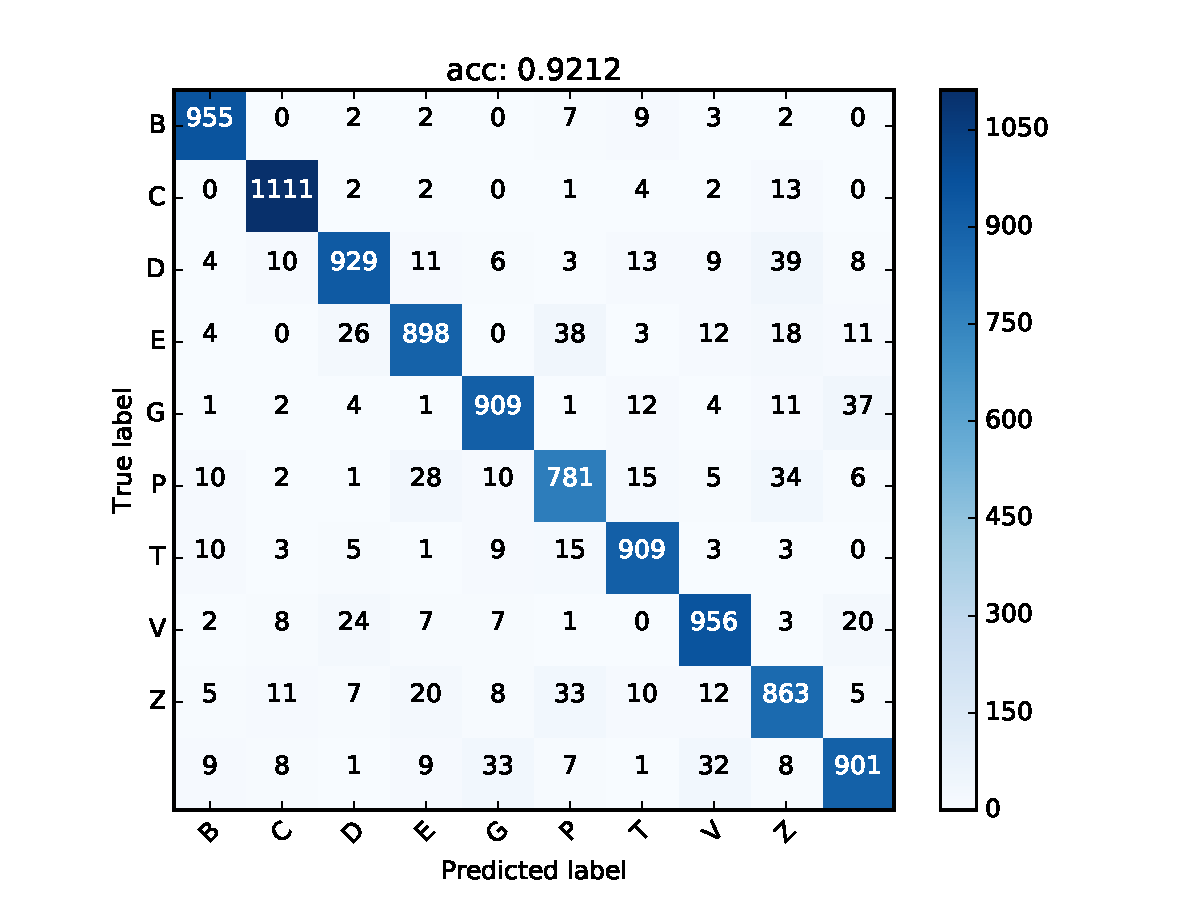
\includegraphics[width = 0.35\textwidth]{../figures/test-pca.pdf}}
      \subfigure[train-rbm-200]
      {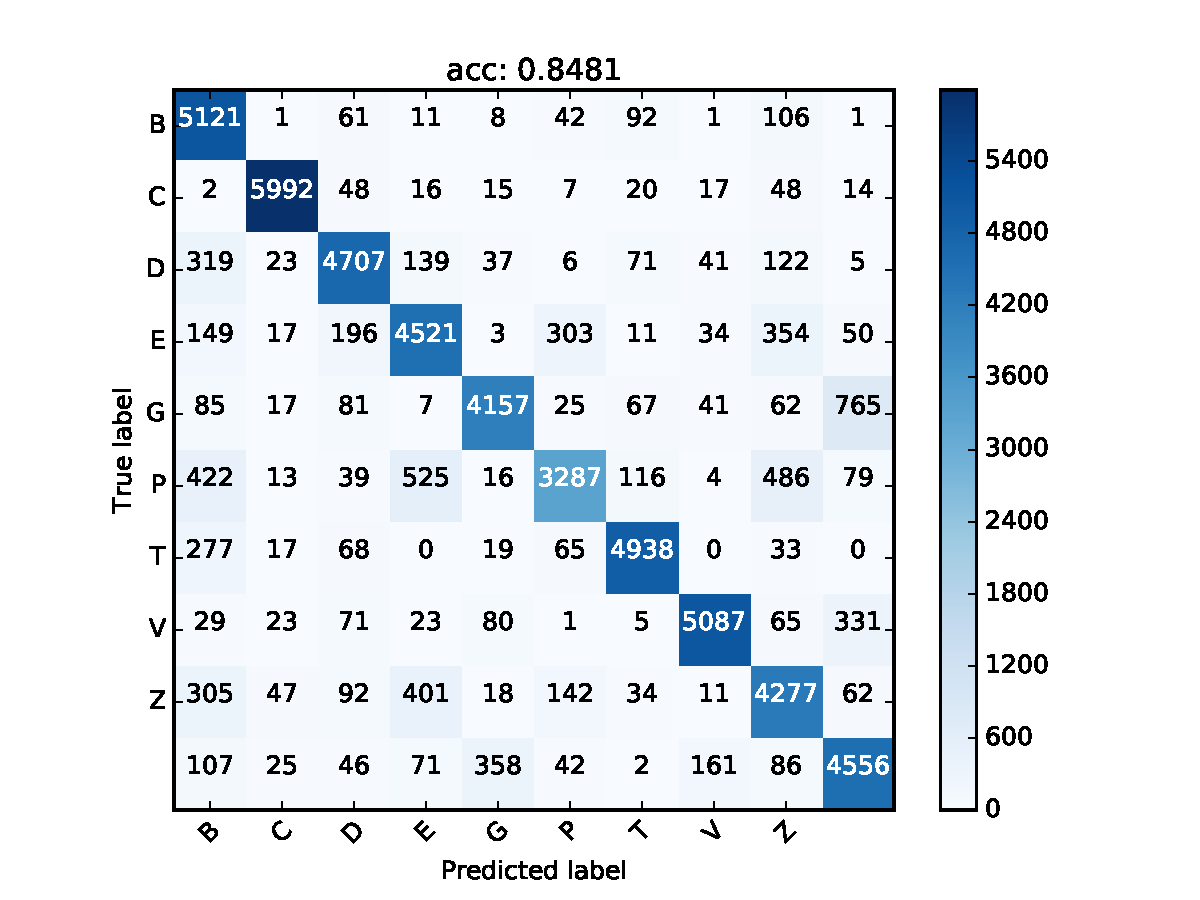
\includegraphics[width = 0.35\textwidth]{../figures/train-rbm-200.pdf}}
      \subfigure[test-rbm-200]
      {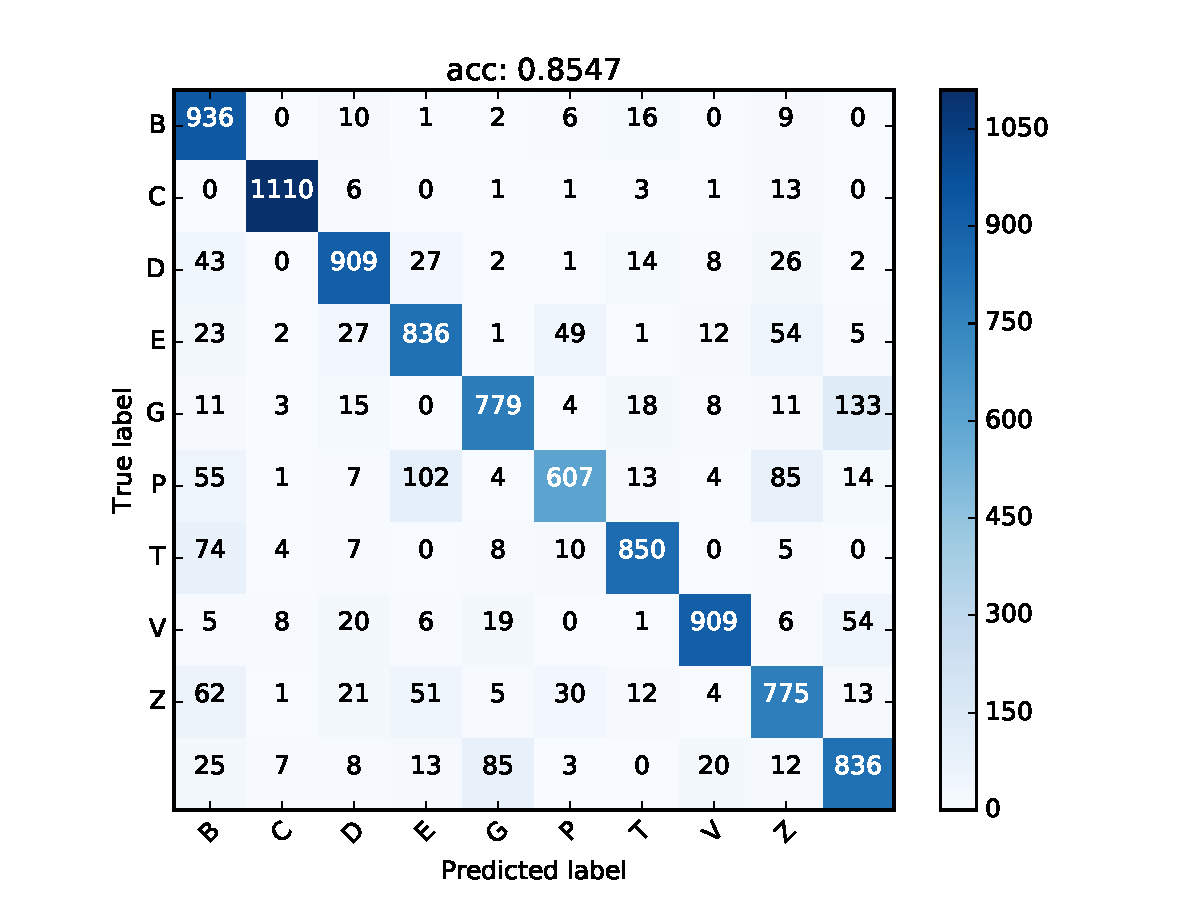
\includegraphics[width = 0.35\textwidth]{../figures/test-rbm-200.pdf}}
      \subfigure[train-rbm-500-200]
      {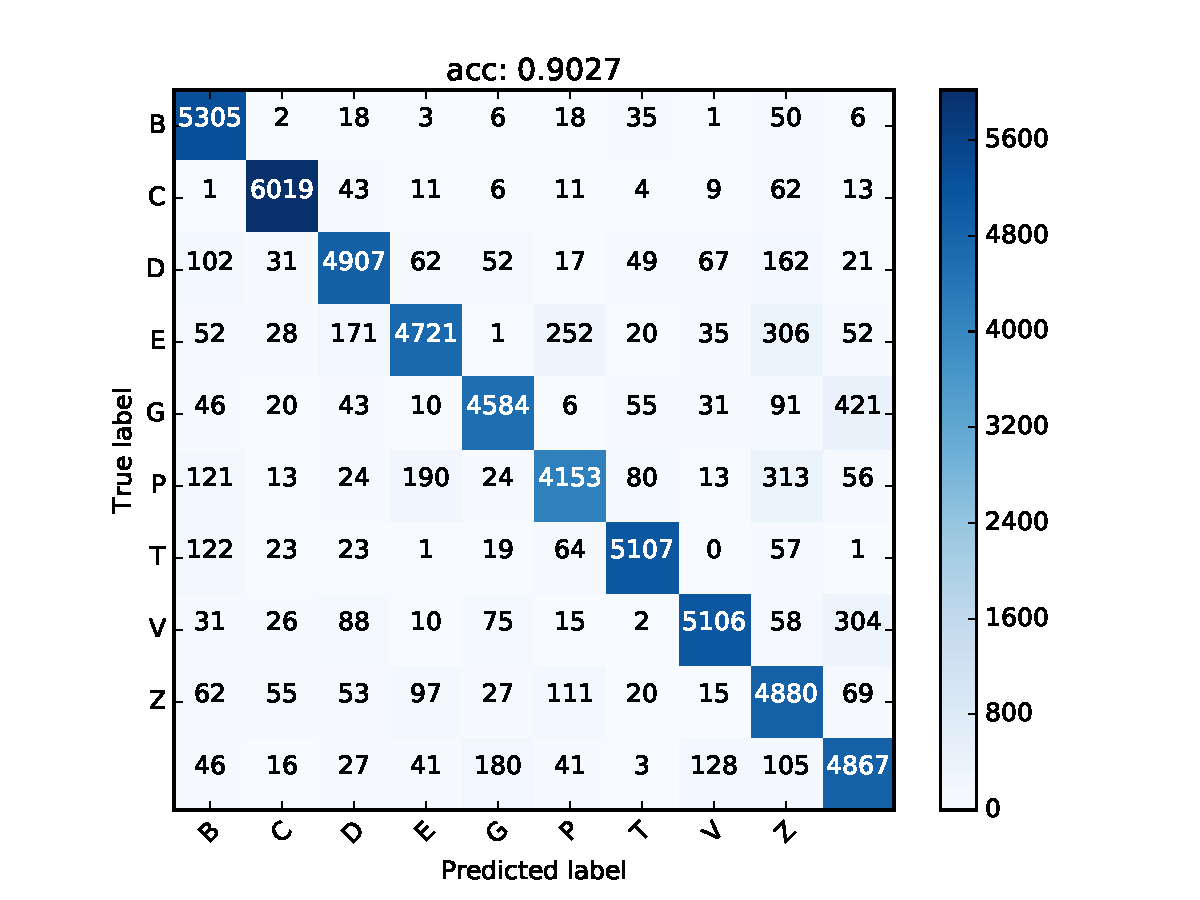
\includegraphics[width = 0.35\textwidth]{../figures/train-rbm-500-200.pdf}}
      \subfigure[test-rbm-500-200]
      {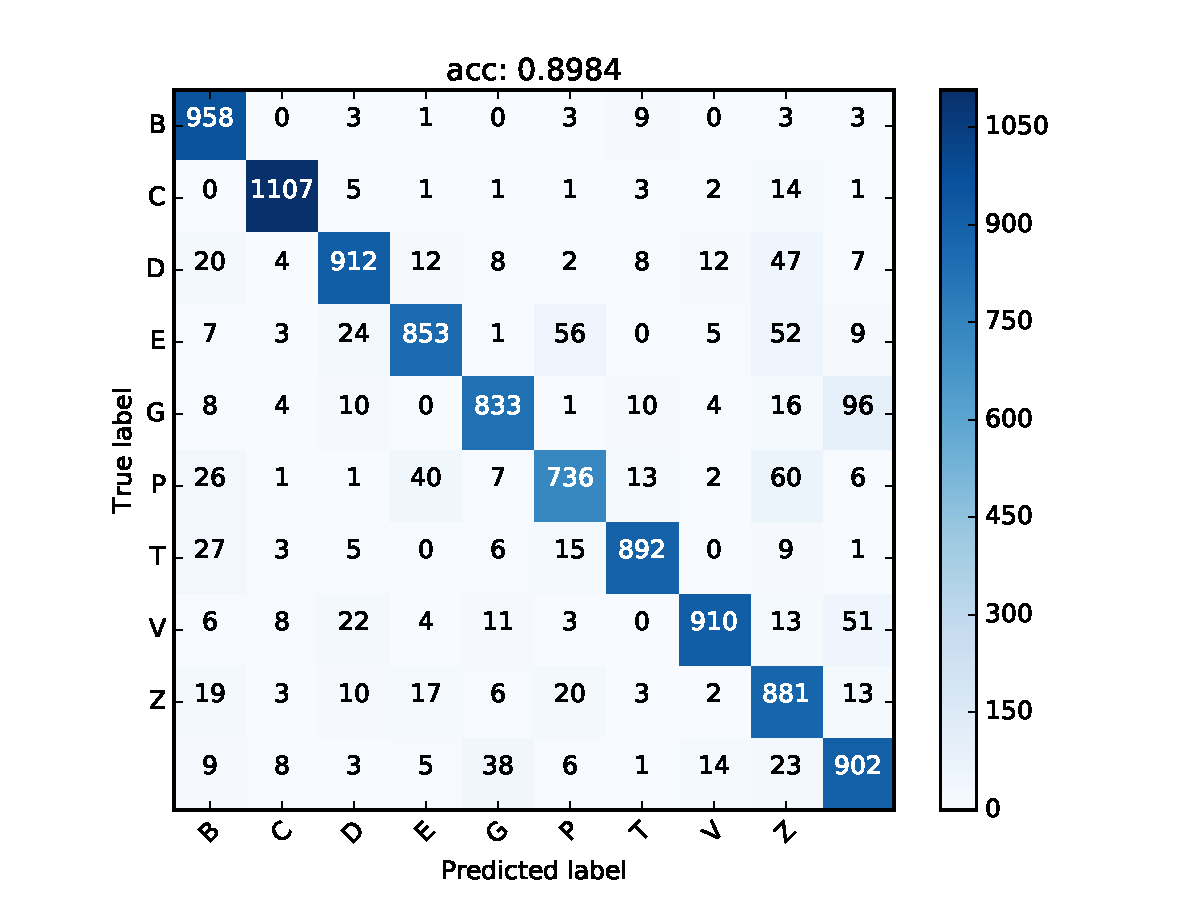
\includegraphics[width = 0.35\textwidth]{../figures/test-rbm-500-200.pdf}}
      \caption{Confusion matrices.\label{fig:part3}}
    \end{figure}
  \end{proof}
\end{itemize}
\par}
\end{document}
